\section{Association Rules}
Questa sezione è dedicata all'\textit{Association Rules Mining}: dopo una prima fase di \textit{data preparation} abbiamo estratto gli \textit{itemset} più frequenti e da questi, attraverso la funzione \textit{Apriori}, ottenuto le regole di associazione. Il nostro obiettivo era quello di trovare delle regole con le quali sostituire i \textit{missing values} presenti nel dataset e costruire un modello predittivo di \textit{Attrition}, la nostra \textit{target variable}.

\subsection{Preparazione dei dati}
Per l'esecuzione delle regole di associazione i dati sono stati preparati come discusso nella sezione di \textit{Data Understanding}, senza però sostituire i \textit{missing values}. Gli attributi quantitativi (\textit{Age} e \textit{MonthlyIncome}) sono stati poi discretizzati nei seguenti intervalli stabiliti osservando i grafici generati con il metodo \textit{KDE} (Fig.\ref{AR}): per \textit{Age} (18.0, 40.0], (40.0, 48.0], (48.0, 62.0], mentre per \textit{MonthlyIncome} (1009.0, 4000.0], (4000.0, 8000.0], (8000.0, 11416.0].
\begin{figure}[H]
	\centering
	\subfloat[] 
	{
		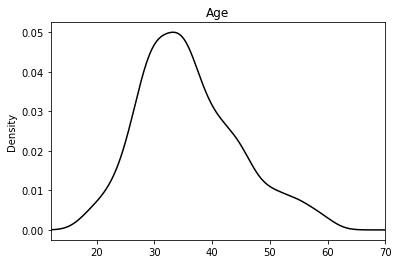
\includegraphics[width=.43\textwidth]{Immagini/kde_Age.png}
		\label{kde_Age}
	}
	\quad
	\subfloat[]
	{
		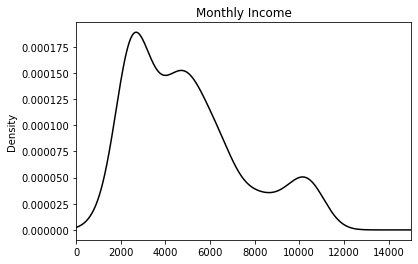
\includegraphics[width =.45\textwidth]{Immagini/kde_MI.png}
		\label{kde_MI}
    }
	\caption{Kernel Density Estimation di Age e MonthlyIncome}
	\label{AR}
\end{figure}
\subsection{\textit{Frequent Itemset}}
Ai dati preparati abbiamo applicato l'algoritmo \textit{Apriori}, con \textit{support} 10\% e lunghezza minima dell'\textit{itemset} 1, per ottenere i \textit{frequent}, i \textit{closed} e i \textit{maximal itemset}. In totale abbiamo ottenuto 431 \textit{frequent} e \textit{closed itemset} e 148 \textit{maximal itemset}. Nelle tabelle Tab. \ref{FrequentItemsets} e Tab. \ref{Maximal Itemsets} abbiamo riportato solo gli itemset con alti valori di \textit{support} (i \textit{frequent itemset} e i \textit{closed itemset} sono identici, e sono stati quindi inseriti nella stessa tabella). L'analisi dei \textit{frequent itemset} evidenzia nuovamente, come già descritto nel \textit{Data Understanding}, che la maggior parte dei lavoratori IBM sono uomini con età compresa tra 18 e 40 anni che possiedono un alto livello di soddisfazione lavorativa e personale e che, dunque, tendono a non licenziarsi. 
\begin{table}[H]
\vspace{3mm}
\centering
\resizebox{.99\textwidth}{!}{
\begin{tabular}{ |p{2cm}|p{10cm}|}
\hline
 \textbf{Support} & \textbf{Frequent-Closed itemsets} \\
 \hline
\textbf{80\% - 90\%}& \textbf{1)} \{Attrition: No\} (\textit{supp} = 0.83)\\
\hline
\textbf{70\% - 80\%}& \textbf{2)} \{OverTime: No\} (\textit{supp} = 0.70)\\
\hline
\textbf{60\% - 70\%}& \textbf{3)} \{OverTime: No, Attrition: No\} (\textit{supp} = 0.63)\\
& \textbf{4)} \{Age: (18.0, 40.0]\} (\textit{supp} = 0.61)\\
& \textbf{5)} \{WorkLifeBalance: High\} (\textit{supp} = 0.60)\\
\hline
\textbf{50\% - 60\%}& \textbf{6)} \{Gender: Male\} (\textit{supp} = 0.57) \\
& \textbf{7)} \{GeneralEmployeeSatisfaction: High\} (\textit{supp} = 0.53)\\
& \textbf{8)} \{WorkLifeBalance: High, Attrition: No\} (\textit{supp} = 0.51)\\
& \textbf{9)} \{Age: (18.0, 40.0], Attrition: No\} (\textit{supp} = 0.50)\\
\hline
\end{tabular}}
\caption{\textit{\textit{Frequent} e \textit{Closed itemset} con un valore di \textit{support} $>$ 50\%}}
\label{FrequentItemsets}
\end{table}
\begin{table}
\centering
\small
\begin{tabular}{ |p{2cm}|p{10cm}|}
\hline
 \textbf{Support} & \textbf{Maximal itemsets} \\
 \hline
\textbf{15\%}& \textbf{1)} \{JobLevel: Low, WorkLifeBalance: High, OverTime: No, Attrition: No\}\\
& \textbf{2)} \{JobLevel: Low, Age: (18.0, 40.0], OverTime: No, Attrition: No\}\\
\hline
\textbf{14\%}& \textbf{3)} \{JobLevel: Very Low, WorkLifeBalance: High, OverTime: No, Attrition: No\}\\
& \textbf{4)} \{Gender: Male, WorkLifeBalance: High, Age: (18.0, 40.0], OverTime: No, Attrition: No\}\\
& \textbf{5)} \{MonthlyIncome: (1009.0, 4000.0], Age: (18.0, 40.0], OverTime: No, Attrition: No\}\\
& \textbf{6)} \{JobLevel: Low, Gender: Male, Overtime: No, Attrition: No\}\\
& \textbf{7)} \{Gender: Female, WorkLifeBalance: High, OverTime: No, Attrition: No\}\\
& \textbf{8)} \{WorkLifeBalance: Medium, Overtime: No, Attrition: No\}\\
& \textbf{9)} \{JobLevel: Very Low, Age: (18.0, 40.0], OverTime: No, Attrition: No\}\\
\hline
\end{tabular}
\caption{\textit{Maximal itemsets ottenuti con min\_support = 0.10}}
\label{Maximal Itemsets}
\end{table}
\subsection{Association Rules}
Dai \textit{frequent itemset} ottenuti abbiamo estratto le regole di associazione impostando una \textit{min\_confidence} del 60\% (regole con \textit{confidence} più bassa, vere cioè meno del 60\% delle volte, sono poco informative). Abbiamo così ottenuto 965 regole. Alcune di esse, come si può notare dai grafici seguenti (Fig. \ref{Confidence}), presentano una \textit{confidence} compresa tra 80\% e 90\%. 
\begin{figure}[H]
	\centering
	\subfloat[] 
	{
		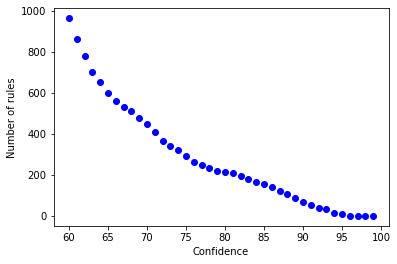
\includegraphics[width=.45\textwidth]{Immagini/confidence.png}
		\label{Conf}
	}
	\quad
	\subfloat[]
	{
		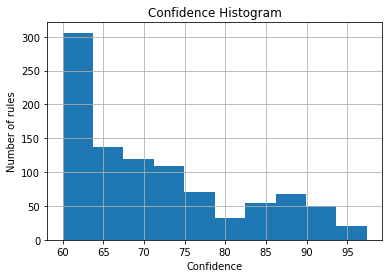
\includegraphics[width =.45\textwidth]{Immagini/hist_conf.png}
		\label{Conf_hist}
    }
	\caption{Distribuzione del numero di regole in base ai valori di \textit{confidence}}
	\label{Confidence}
\end{figure}
\noindent 
Per quanto riguarda il \textit{lift} (Fig. \ref{lift}), la sua distribuzione è sbilanciata verso il valore di 1: vi sono, quindi, molte regole i cui elementi sono associati tra loro in maniera casuale. Solo un piccolissimo numero di regole ha lift compreso tra 1.6 e 1.9. 
\begin{figure}[H]
    \centering
    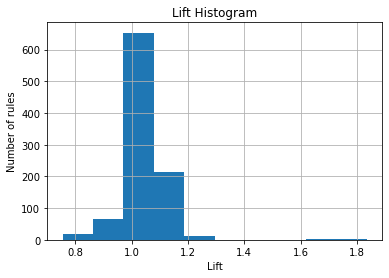
\includegraphics[scale=0.5]{Immagini/lift.png}
    \caption{Distribuzione del numero di regole in base ai valori di lift}
    \label{lift}
\end{figure}
\noindent Delle 965 regole abbiamo selezionato le più informative. Per il principio di anti-monotonicità su cui si basa l'algoritmo \textit{Apriori}, riportiamo successivamente solo 8 regole, ordinate secondo il parametro di lift, generate da diversi itemset.
\begin{table}[H]
\centering
\small
\begin{tabular}{|p{15cm}|}
\hline
 \textbf{Association Rules} \\
 \hline
\{Attrition: Yes, Age: (18.0, 40.0]\} $=>$ JobLevel: Very Low (\textit{conf} = 0.71) (\textit{lift} = 1.83)\\
\hline
\{MonthlyIncome: (1009.0, 4000.0], Marital Status: Married\} $=>$ Age: (18.0, 40.0] (\textit{conf} = 0.74) (\textit{lift} = 1.21)\\
\hline
\{JobLevel: Very Low, Gender: Male, WorkLifeBalance: High, Attrition: No\} $=>$ OverTime: No (\textit{conf} = 0.86) (\textit{lift} = 1.21)\\
\hline
\{MonthlyIncome: (1009.0, 4000.0], JobLevel: Very Low\} $=>$ Age: (18.0, 40.0] (\textit{conf} = 0.74) (\textit{lift} = 1.21)\\
\hline
 \{OverTime: Yes, Gender: Male, Attrition: No\} $=>$ GeneralEmployeeSatisfaction: High (\textit{conf} = 1.83) (\textit{lift} = 0.64)\\
\hline
\{JobLevel: Low, GeneralEmployeeSatisfaction: High, Age: (18.0, 40.0]\} $=>$ Attrition: No (\textit{conf} = 0.97) (\textit{lift} = 1.17)\\
\hline
\{Gender: Male, WorkLifeBalance: High, Age: (18.0, 40.0], OverTime: No\} $=>$ Attrition: No (\textit{conf} = 0.95) (\textit{lift} = 1.15)\\
\hline
\{GeneralEmployeeSatisfaction: Medium, MonthlyIncome: (1009.0, 4000.0]\} $=>$ Gender: Male (\textit{conf} = 0.64) (\textit{lift} = 1.12)\\
\hline
\end{tabular}
\caption{\textit{Association Rules più interessanti, ordinate per valore di lift}}
\label{ARinteressanti}
\end{table}
\noindent Osservando queste regole possiamo affermare che circa il 96\% dei lavoratori IBM non si licenzia e nell'86\% dei casi non fa straordinari. Con probabilità del 75\%, i dipendenti hanno età compresa tra 18 e 40 anni e sono uomini nel 64\% dei casi. La quinta regola, infine, evidenzia che nel 64\% dei casi i lavoratori sono molto soddisfatti del loro lavoro (dimostrando che la nuova \textit{feature} da noi creata (\textit{GeneralEmployeeSatisfaction}) è risultata utile nelle analisi). 
\subsection{Sostituzione dei \textit{missing values}}
Dopo aver estratto le regole più interessanti, abbiamo sostituito i valori mancanti di \textit{Age}, \textit{MonthlyIncome} e \textit{Gender}.
\begin{itemize}
\item \textit{Age} presentava 168 \textit{missing values} e con le regole estratte (con \textit{confidence} compresa tra 60\% e 75\%) siamo riusciti a sostituirne 89 con il valore (18.0, 40.0]. Gli altri intervalli d'età presentavano una \textit{confidence} minore nel 60\% e non sono stati considerati validi per la sostituzione;
\item \textit{MonthlyIncome} aveva 213 \textit{missing values} che non siamo riusciti a sostituire in quanto le prime regole utili per la sostituzione hanno tutte una \textit{confidence} del 40\%;
\item \textit{Gender} aveva 51 \textit{missing values} e con le regole estratte (con \textit{confidence} compresa tra 60\% e 64\%) siamo riusciti a sostituirne 40 con il valore \textit{Male}. Per il valore di \textit{Female} non abbiamo trovato regole con una \textit{confidence} maggiore del 60\%.
\end{itemize}
\subsection{Predizione della \textit{target variable}}
Abbiamo usato le regole estratte per costruire un modello predittivo per la nostra \textit{target variable}. L'accuratezza del modello è del 94\%. Sebbene possa apparire un ottimo risultato, il modello assegna sempre e solo il valore di \textit{Attrition: No} dal momento che non vi sono regole con \textit{confidence} maggiore del 60\% che hanno come conseguenza \textit{Attrition: Yes}.\\\\
Tuttavia abbiamo deciso di rilanciare il modello includendo la prima regola che comprendesse \textit{Attrition: Yes}, che presenta \textit{confidence} pari a 57\%, un valore di poco minore di 60\%. La nuova accuratezza è risultata dell'82\%, ancora un valore alto, ma a causa del forte sbilanciamento dei dati il modello ha continuato ad associare solo il valore di \textit{Attrition: No}.





